\documentclass[10pt]{article}
\usepackage[latin1]{inputenc}
\usepackage{amsmath}
\usepackage{amsfonts}
\usepackage{amssymb}
\usepackage{graphicx}
\usepackage[margin=1in]{geometry}
\usepackage{siunitx}

\usepackage{float}
\usepackage{subcaption}

\title{EELE 582 Optical Design \\ Homework 6 \\ Problem 1 \\ Optimizing a Transmission Sphere }
\author{Roy Smart}
\begin{document}
	
\maketitle	

\section{Introduction}

We are tasked with designing a transmission sphere for use in interferometric testing using as few optical elements as possible. A transmission sphere is a lens optimized for on axis performance with the special characteristic that rays emanating from the last surface are normal to that surface. This document details our procedure to design a transmission sphere in Zemax.

\section{Initial Design}

For our initial design, we started with just a single lens. The thickness was set to 0.5" and the diameter to 4". The curvature of the front surface was found by assuming the lens was equiconvex.
\begin{align*}
	R_1 &=2 (n - 1) f_E \\
	&= 2 (1.5168 - 1) (\SI{792.48}{\milli\meter}) \\
	&= \SI{816.396}{\milli\meter}
\end{align*}
For the last surface, the thickness was found by solving where the marginal ray was zero (M-solve). The curvature was set by solving for where the marginal ray was normal to the surface (N-solve).

This resulted in an optical system that had an effective focal length well over the target value of \SI{792.48}{\milli\meter}. We will use the optimizer from here to get the desired optical parameters.

\begin{figure}[h!]
	\centering
	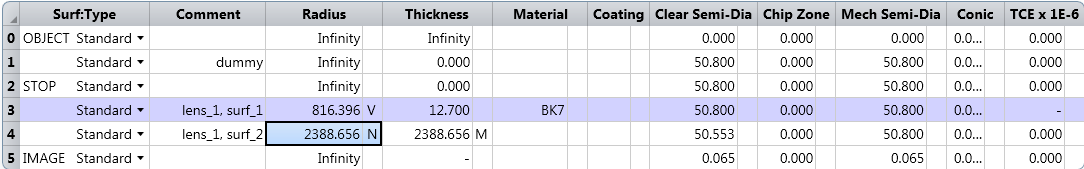
\includegraphics[width=0.75\linewidth]{../zemax/1_oneElement/1_initial/lens.PNG}
	\caption{Initial lens prescription before optimization}
\end{figure}
\begin{figure}[h!]
	\centering
	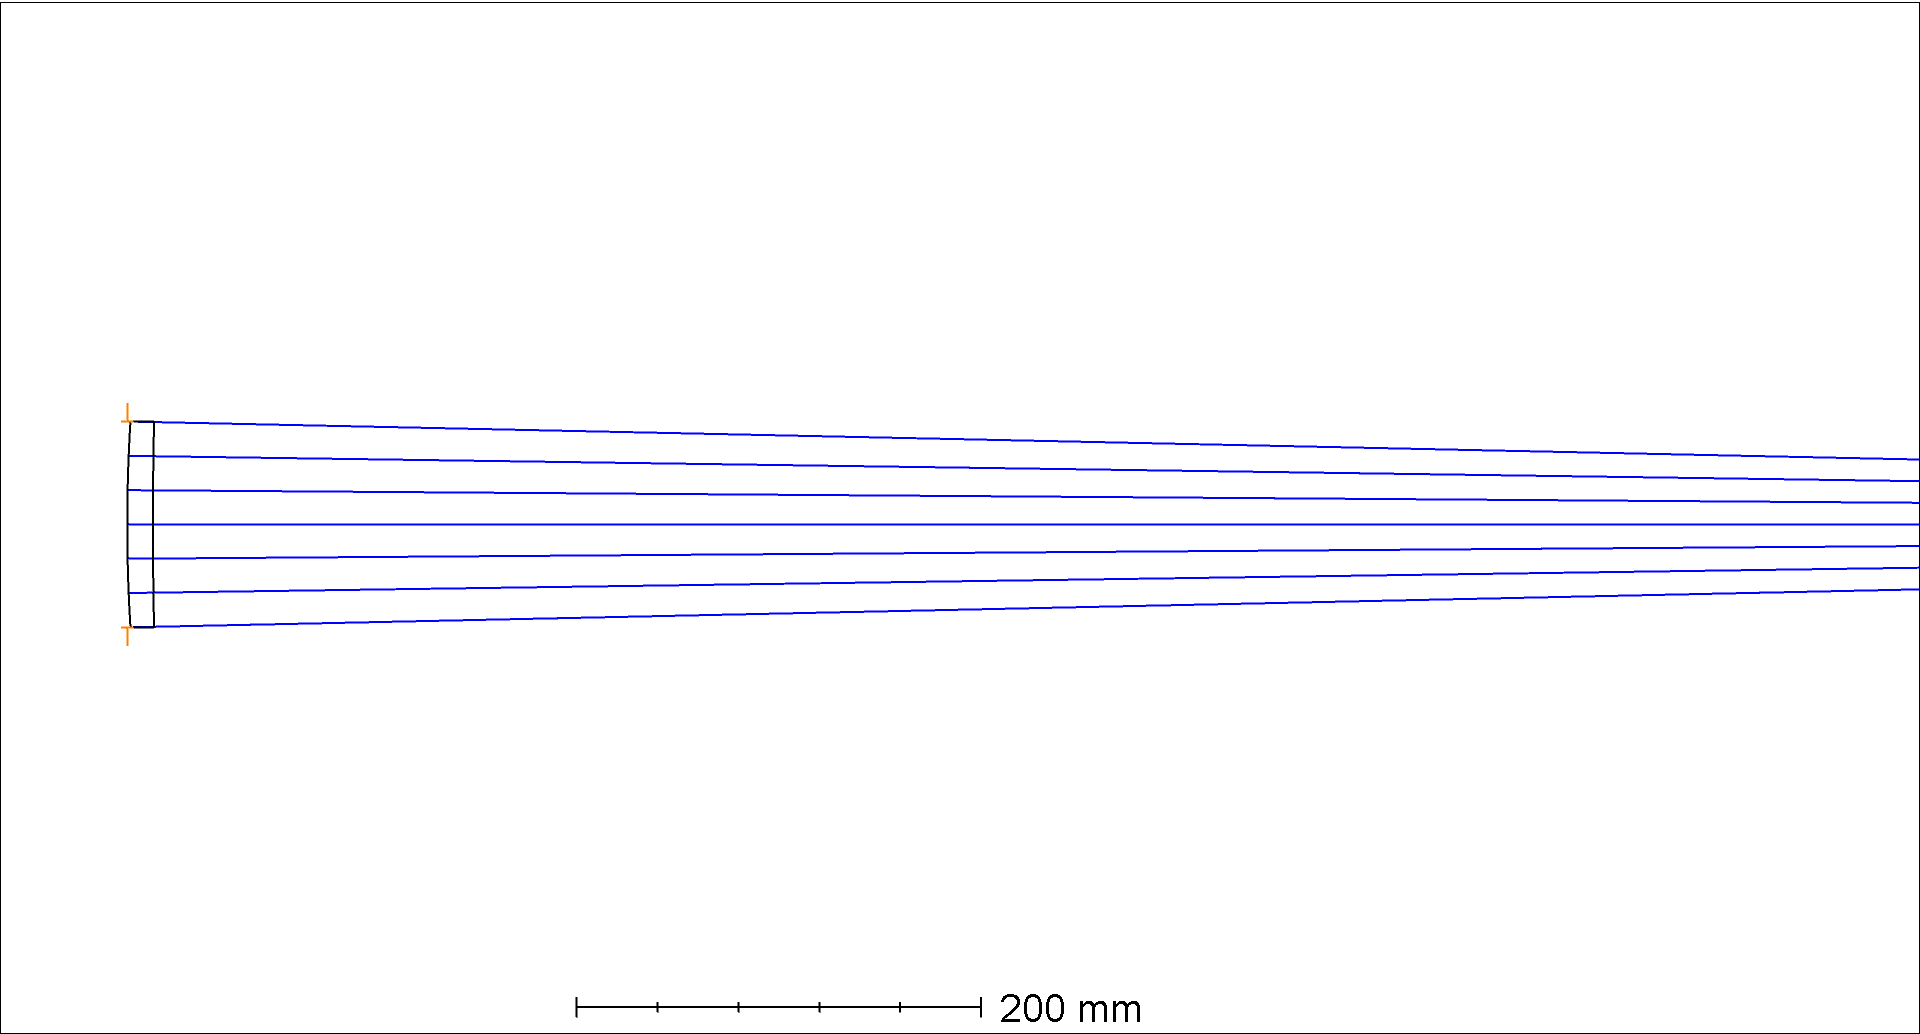
\includegraphics[width=0.75\linewidth]{../zemax/1_oneElement/1_initial/layout.png}
	\caption{Initial lens layout before optimization}
\end{figure}
\section{Merit Function}
We adopted a merit function as suggested by Geary in the problem statement. We used the default merit function to produce the list of \texttt{TRAC} operands to minimize the RMS spot size. We used the \texttt{EFFL} command to reach the target effective focal length. To set the back focal length, we used two \texttt{OPTH} operands to measure the distance to the back surface of the lens and the image plane, respectively. Then a \texttt{DIFF} operand was applied to the return values of the \texttt{OPTH} operands to evaluate the back focal length of the system. The weight of this \texttt{DIFF} operand was set to 1.0 and the value equal to the effective focal length.

\begin{figure}[h!]
	\centering
	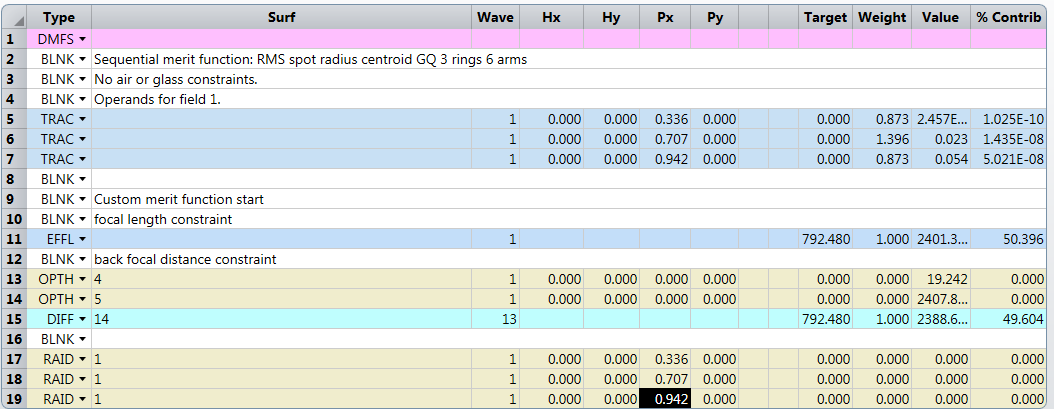
\includegraphics[width=0.75\linewidth]{../zemax/1_oneElement/1_initial/merit.PNG}
	\caption{Merit function evaluated on the initial lens system}
\end{figure}
\section{Optimization}

We adopted an optimization scheme slightly different from the one Geary suggests. In the problem statement, Geary states that the N-solve should be only used as a final optimization step. Here we propose to do it all in a single step, to reduce the number of optimization runs. Furthermore, we will also adopt a lens splitting paradigm where when a lens is split, the two new lenses are taken to have thickness and an air gap of the value given in the problem statement. This paradigm will undoubtedly result in messing with the merit of the optical system slightly, but we will rely on the optimizer to achieve good results. 
\begin{table}[h!]
	\centering
	\begin{tabular}{|r|l|c|c|r|r|}
		\hline
		Lenses & State & Layout & Spot Diagram & EFFL & Spot Size \\ \hline
		1 & initial & 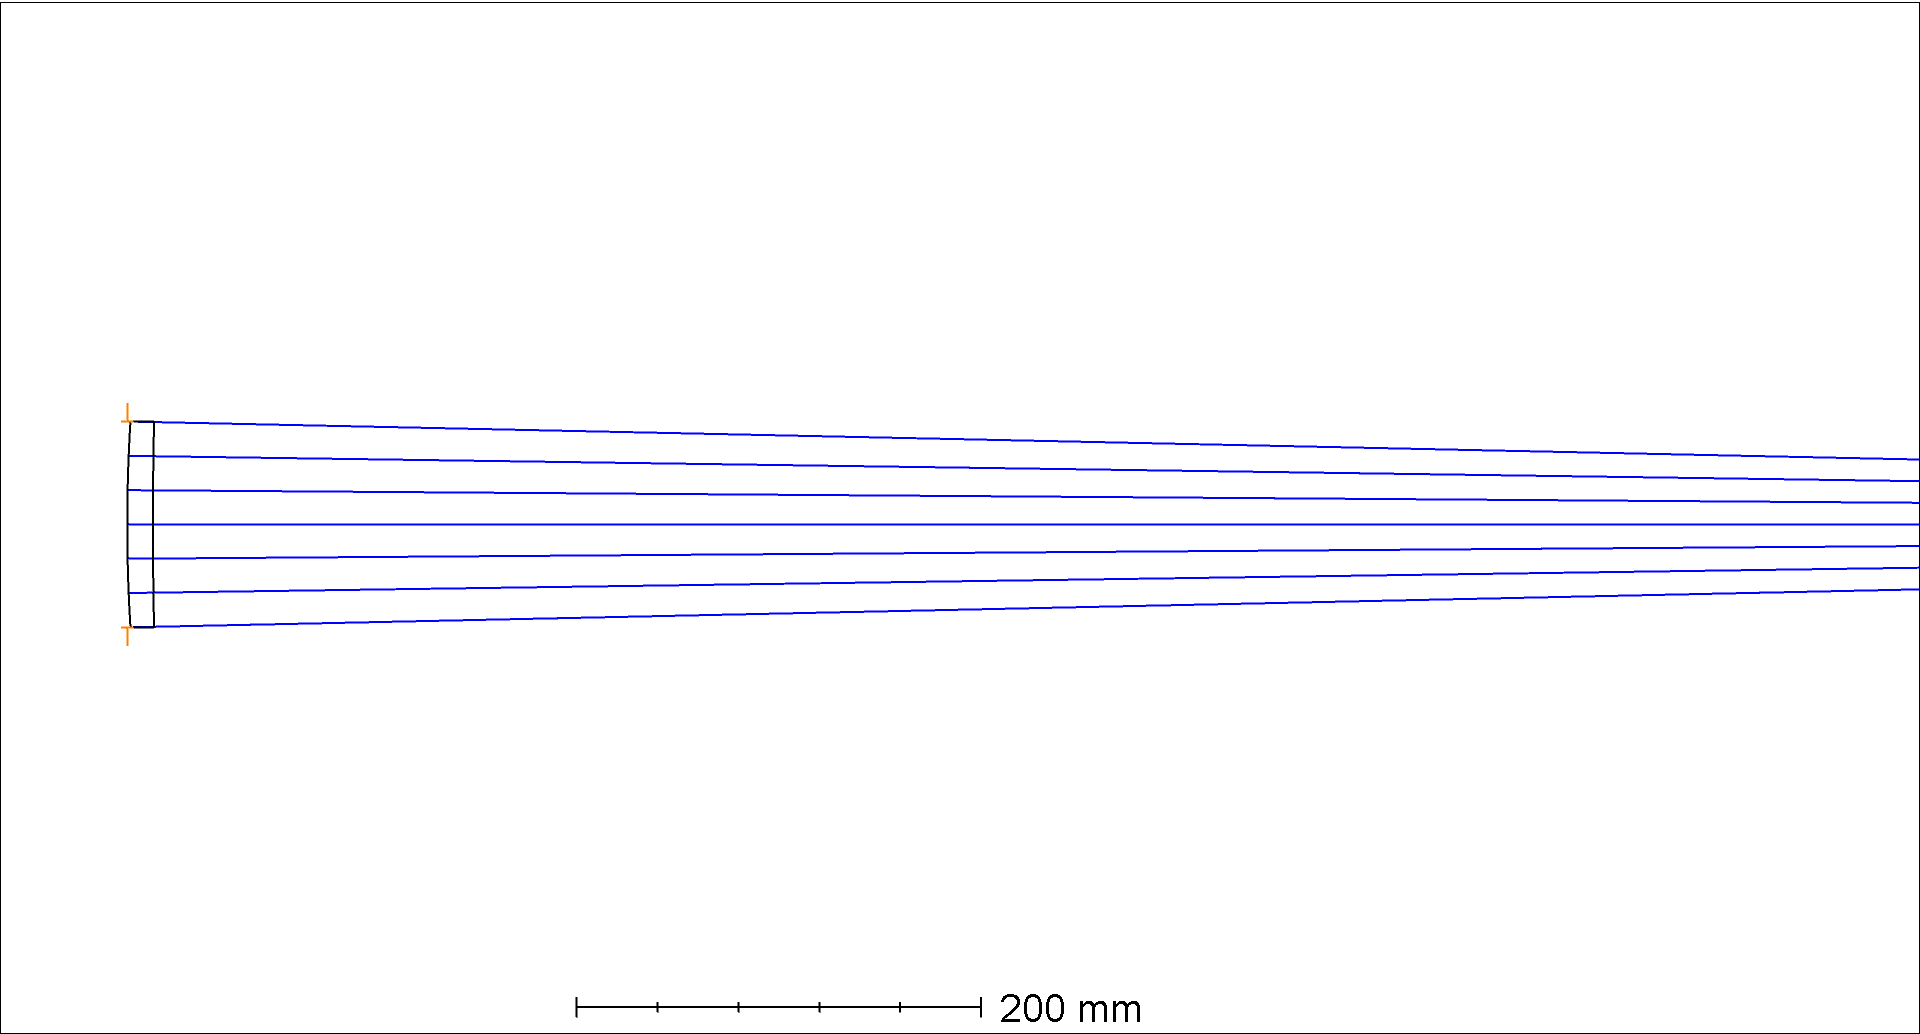
\includegraphics[trim={0.8cm 10cm 40cm 10cm}, clip,height=2.5cm]{../zemax/1_oneElement/1_initial/layout.png} &	
		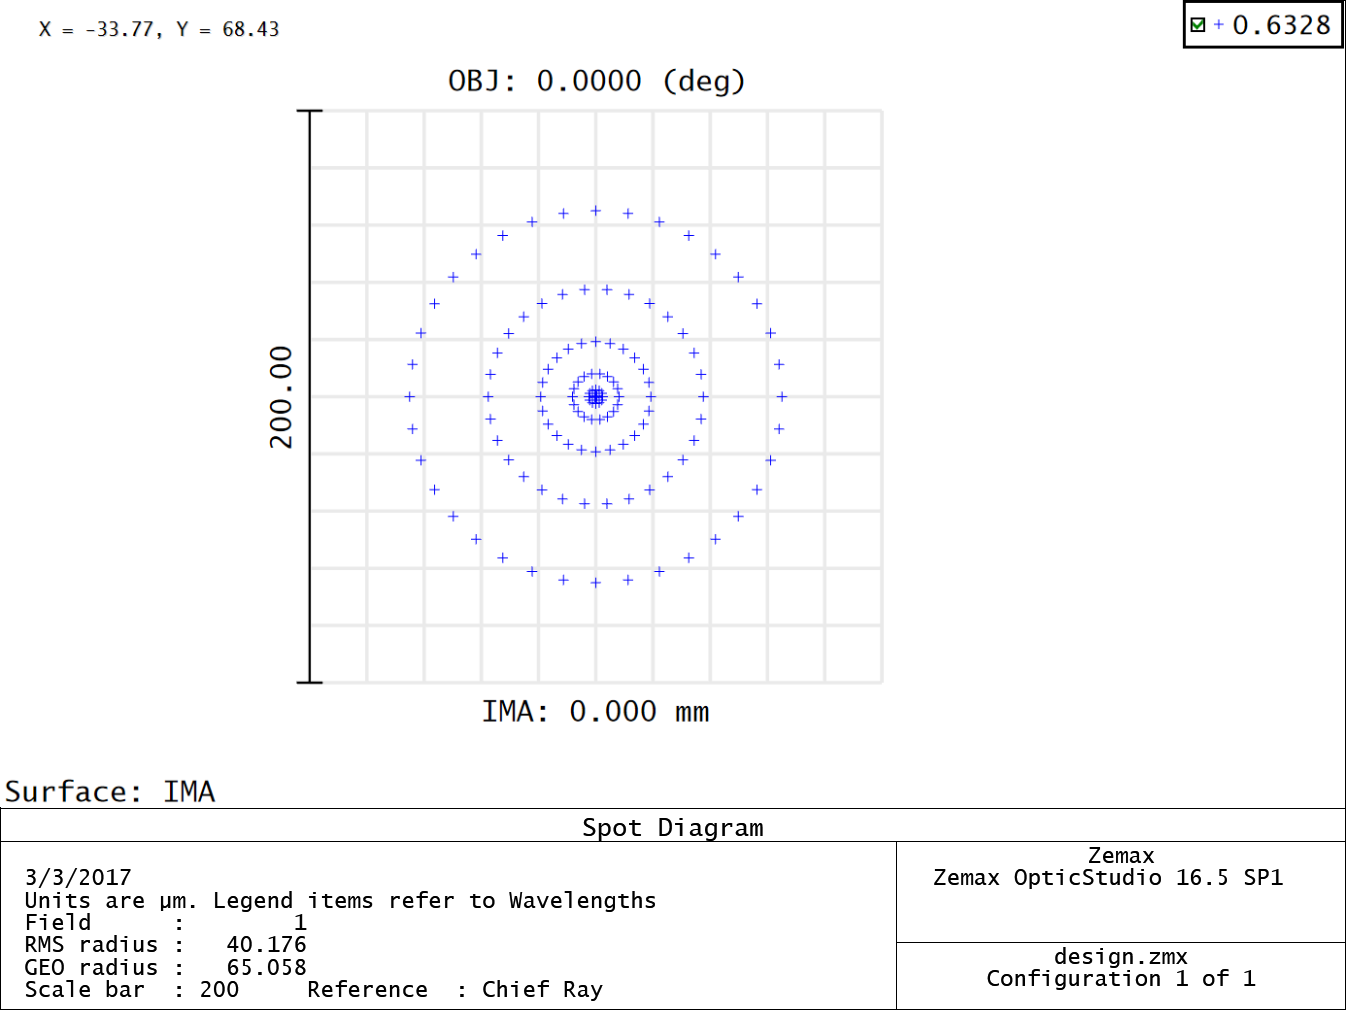
\includegraphics[trim={7.1cm 8.5cm 12cm 2.6cm}, clip,height=2.5cm]{../zemax/1_oneElement/1_initial/spot.png} &  \SI{2401}{\milli \meter} &  \SI{40.1}{\micro \meter} \\\hline
		1 & optimized & 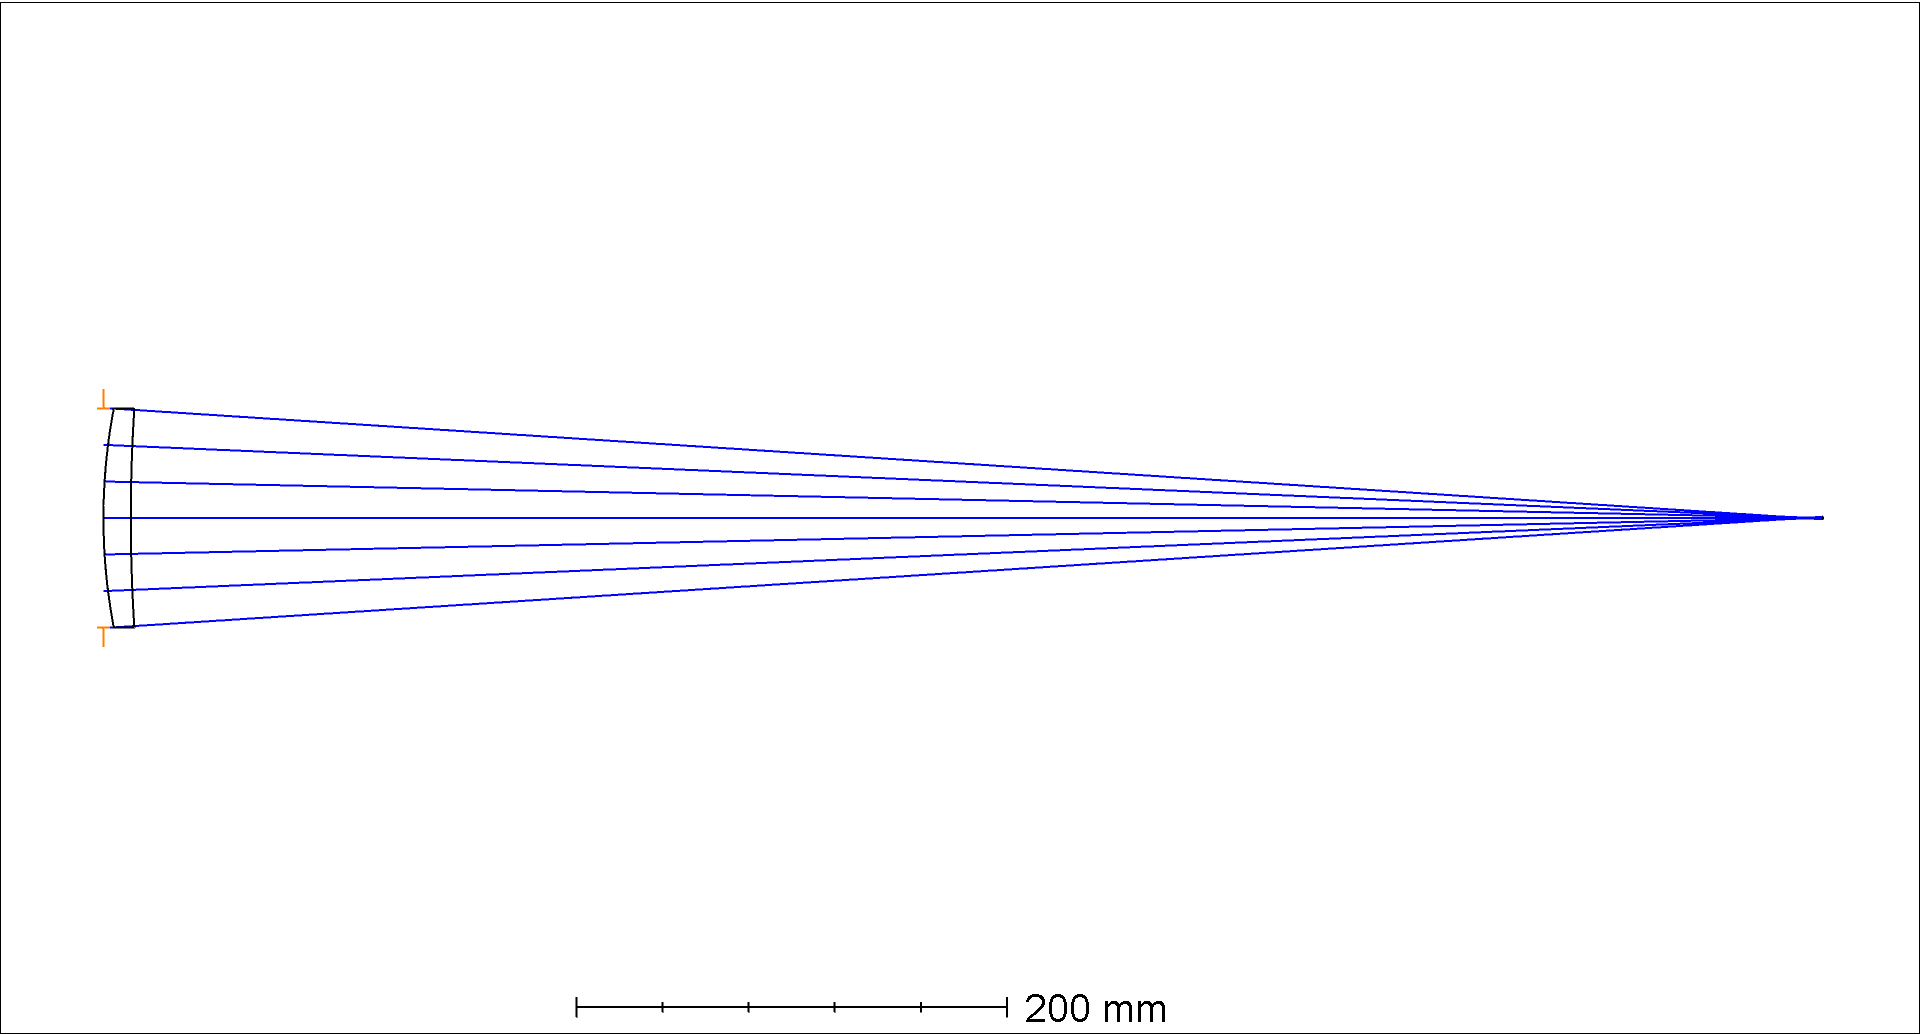
\includegraphics[trim={0.1cm 10cm 40cm 10cm}, clip,height=2.5cm]{../zemax/1_oneElement/2_optimize_RMS/layout.png} & 
		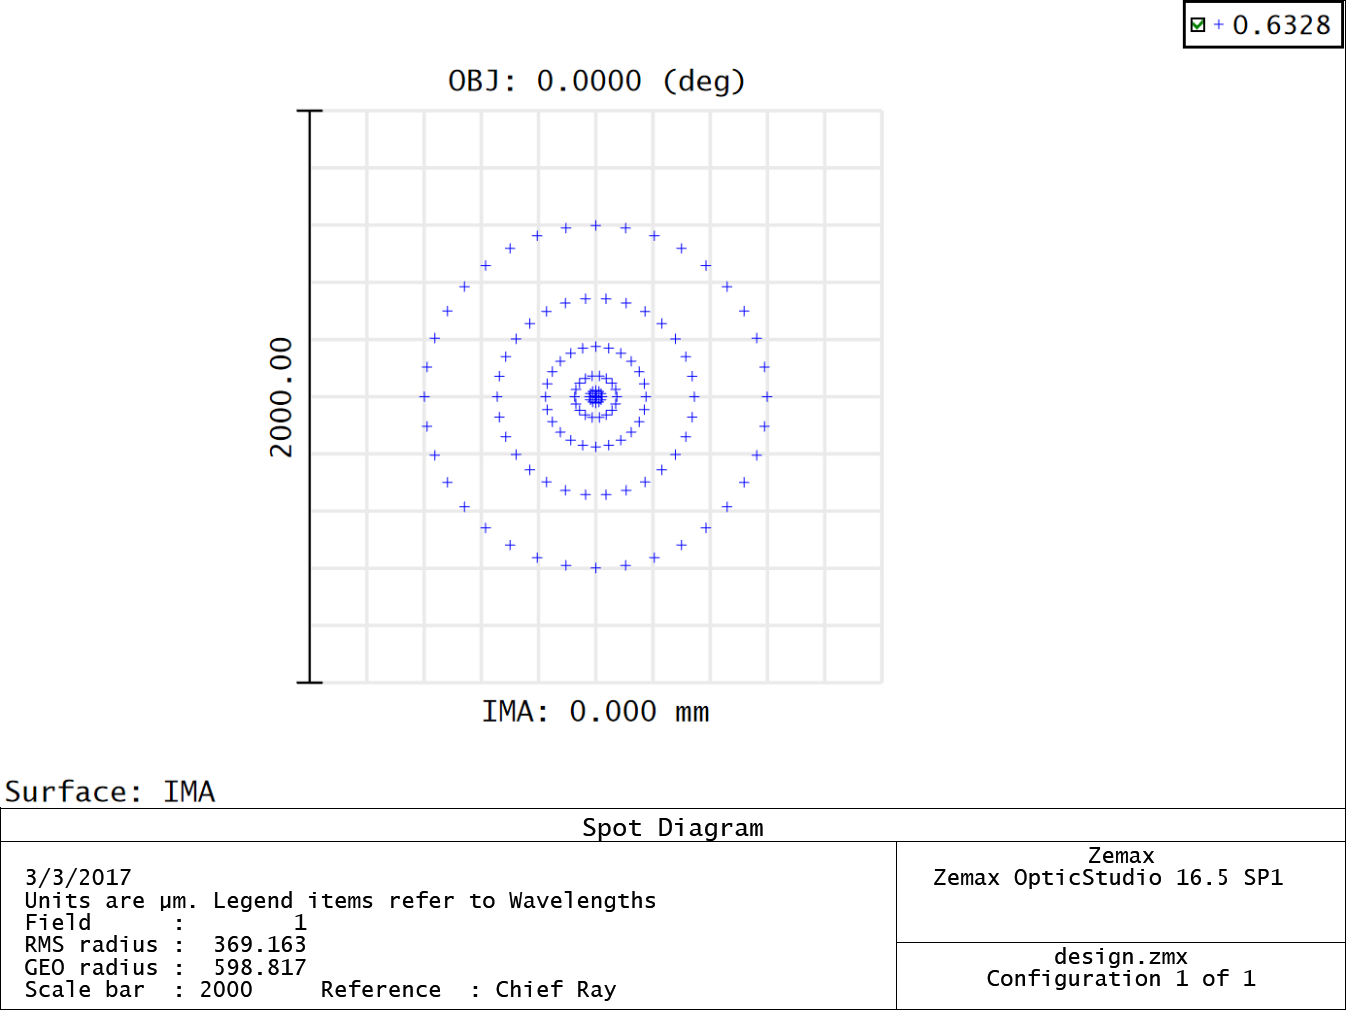
\includegraphics[trim={7.1cm 8.5cm 12cm 2.6cm}, clip,height=2.5cm]{../zemax/1_oneElement/2_optimize_RMS/spot.png} &  \SI{798}{\milli \meter} &  \SI{369}{\micro \meter}\\\hline
		2 & split & 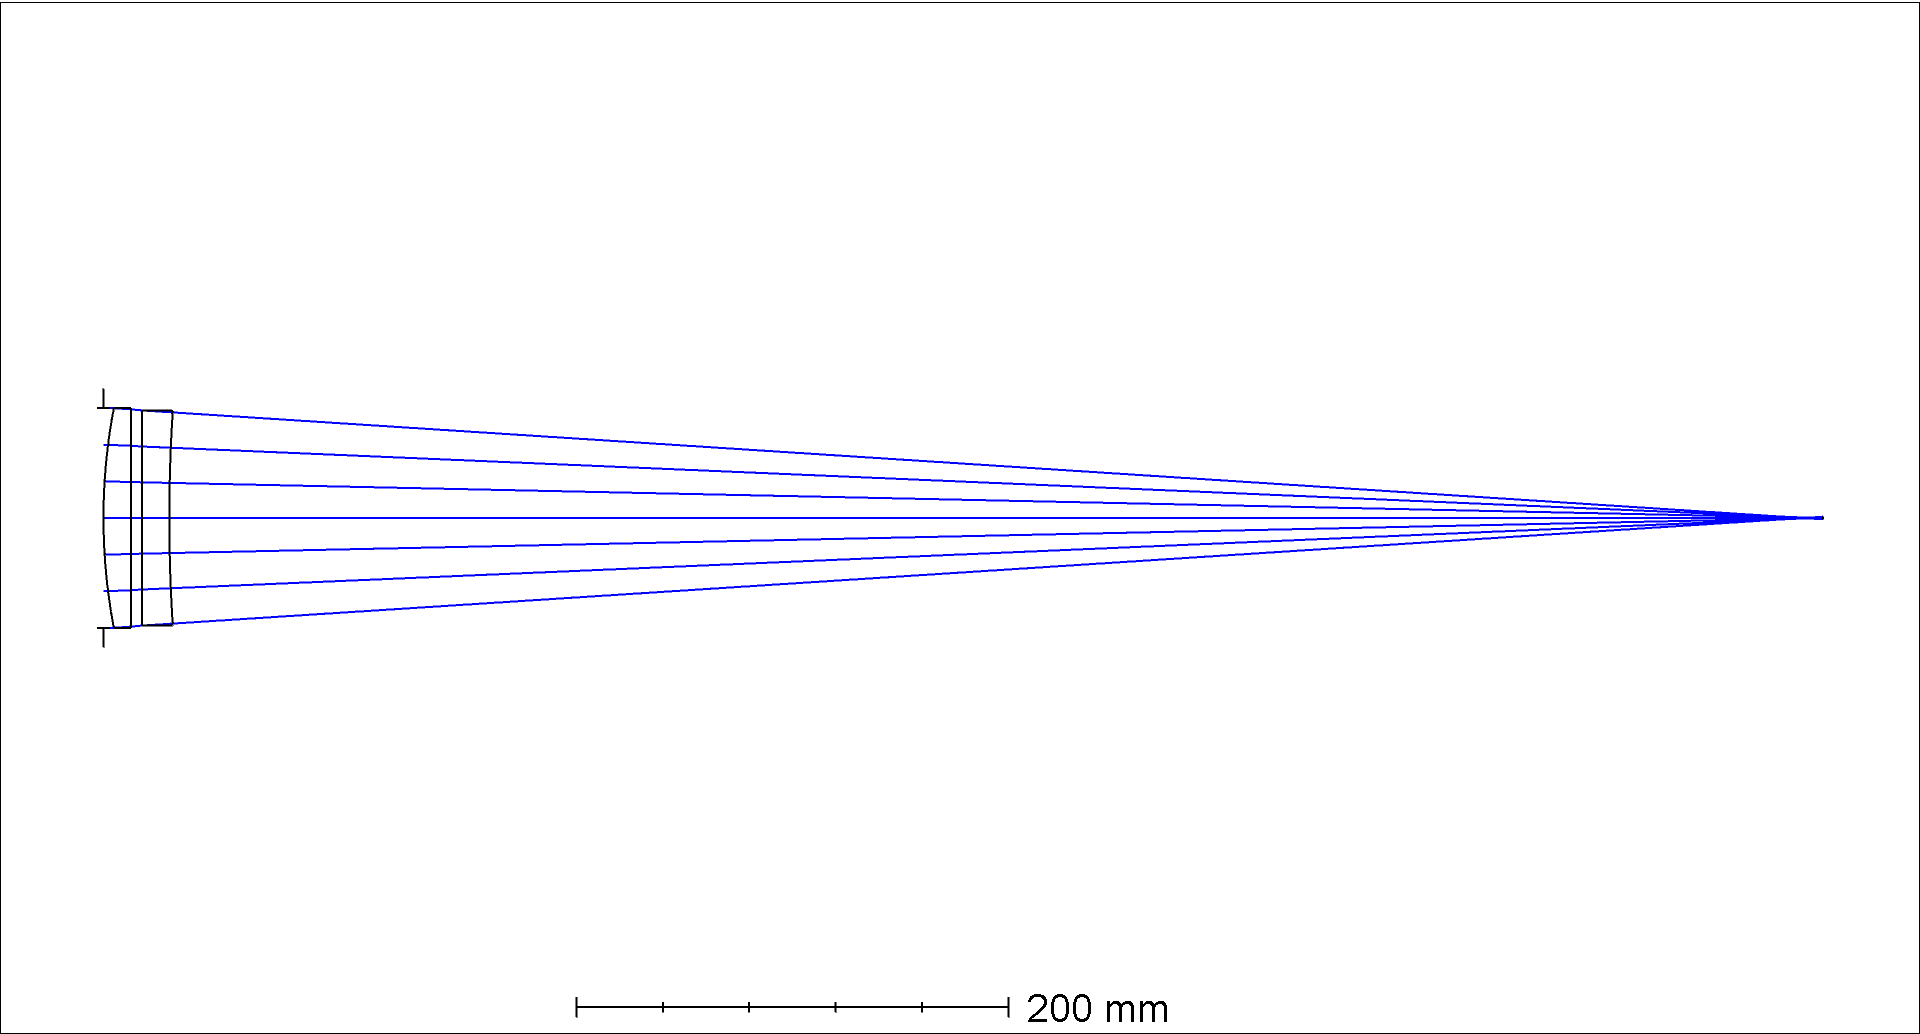
\includegraphics[trim={0.1cm 10cm 40cm 10cm}, clip,height=2.5cm]{../zemax/2_twoElement/1_initial/layout.png} & 
		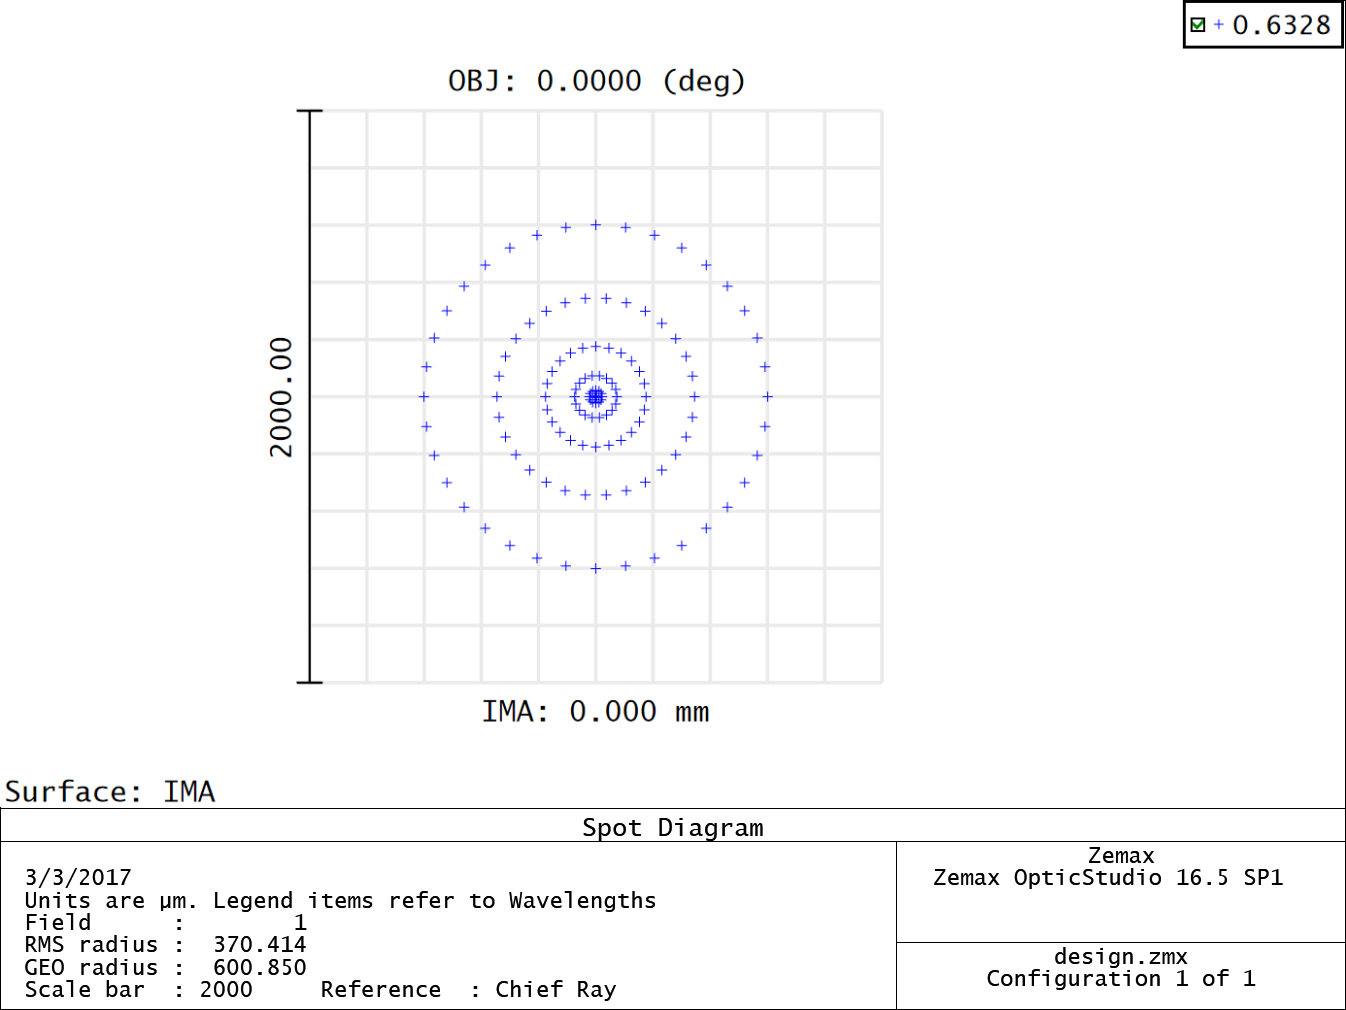
\includegraphics[trim={7.1cm 8.5cm 12cm 2.6cm}, clip,height=2.5cm]{../zemax/2_twoElement/1_initial/spot.png} & \SI{799}{\milli \meter} &  \SI{370}{\micro \meter} \\\hline
		2 & optimized & 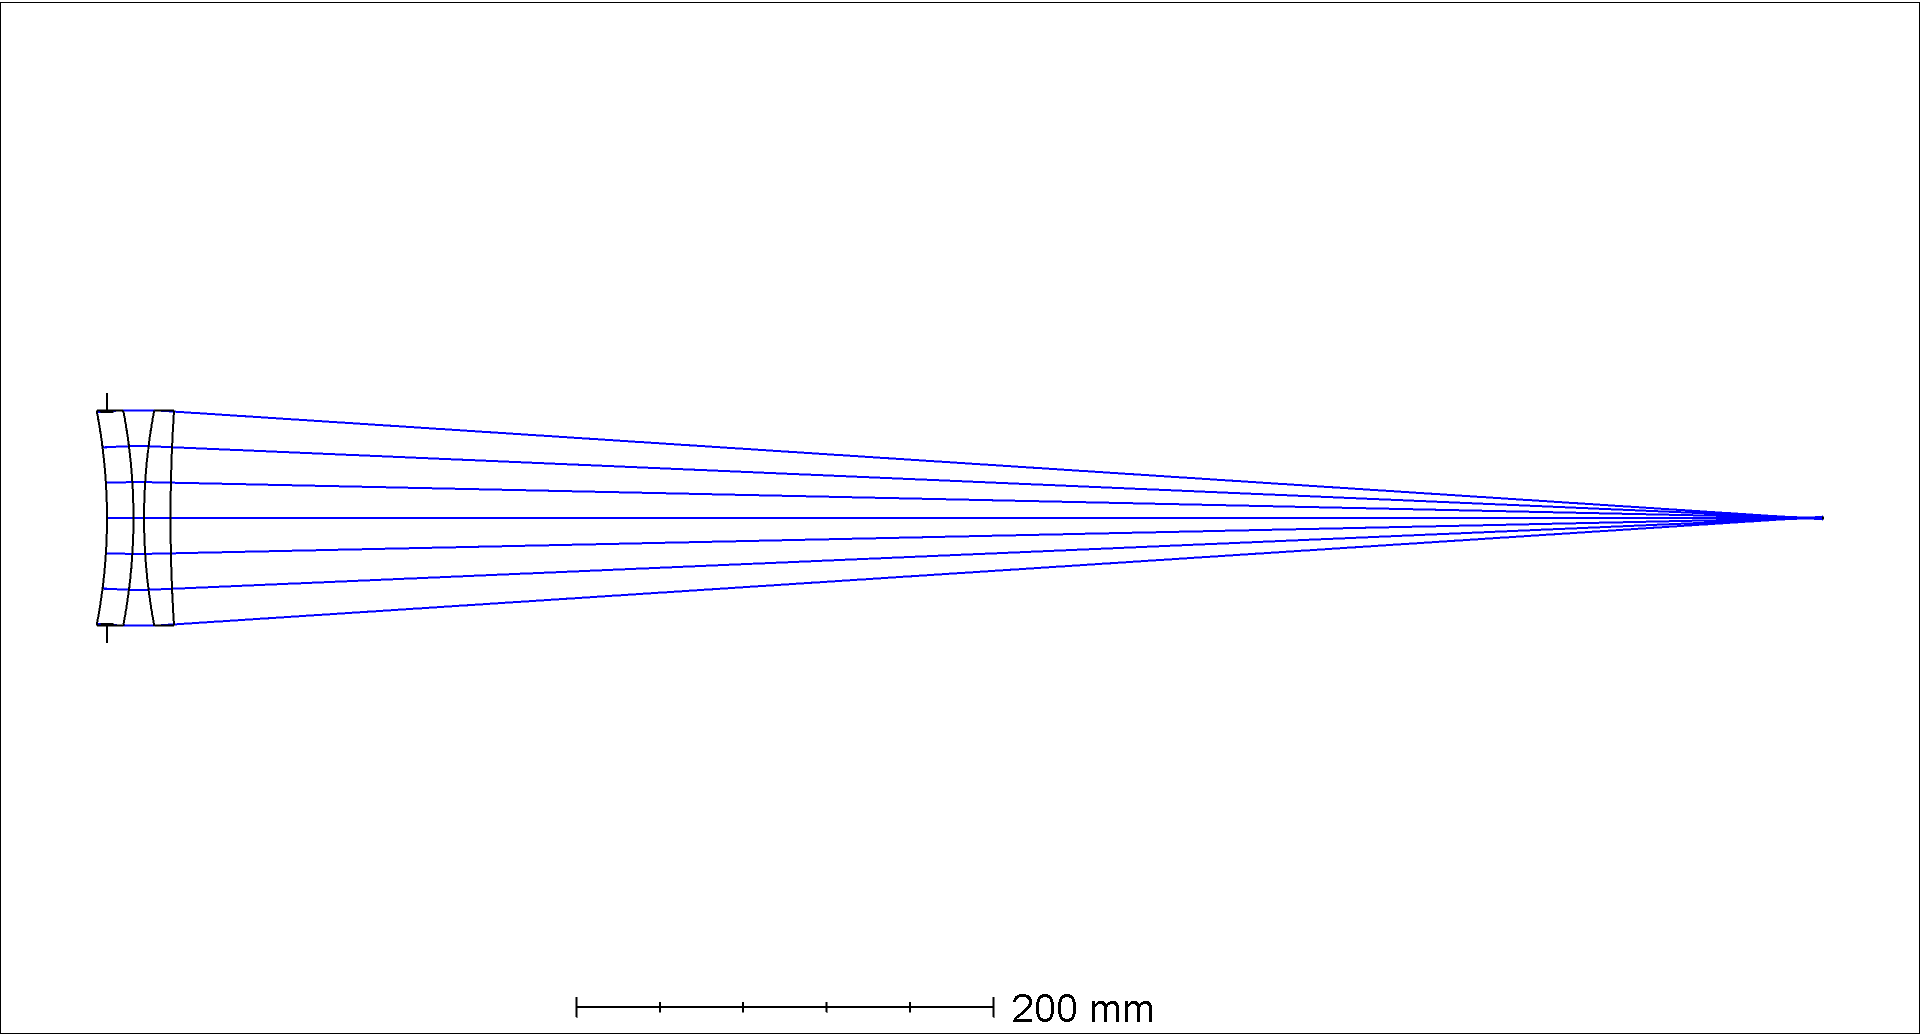
\includegraphics[trim={0.25cm 10cm 40cm 10cm}, clip,height=2.5cm]{../zemax/2_twoElement/2_optimize_RMS/layout.png} & 
		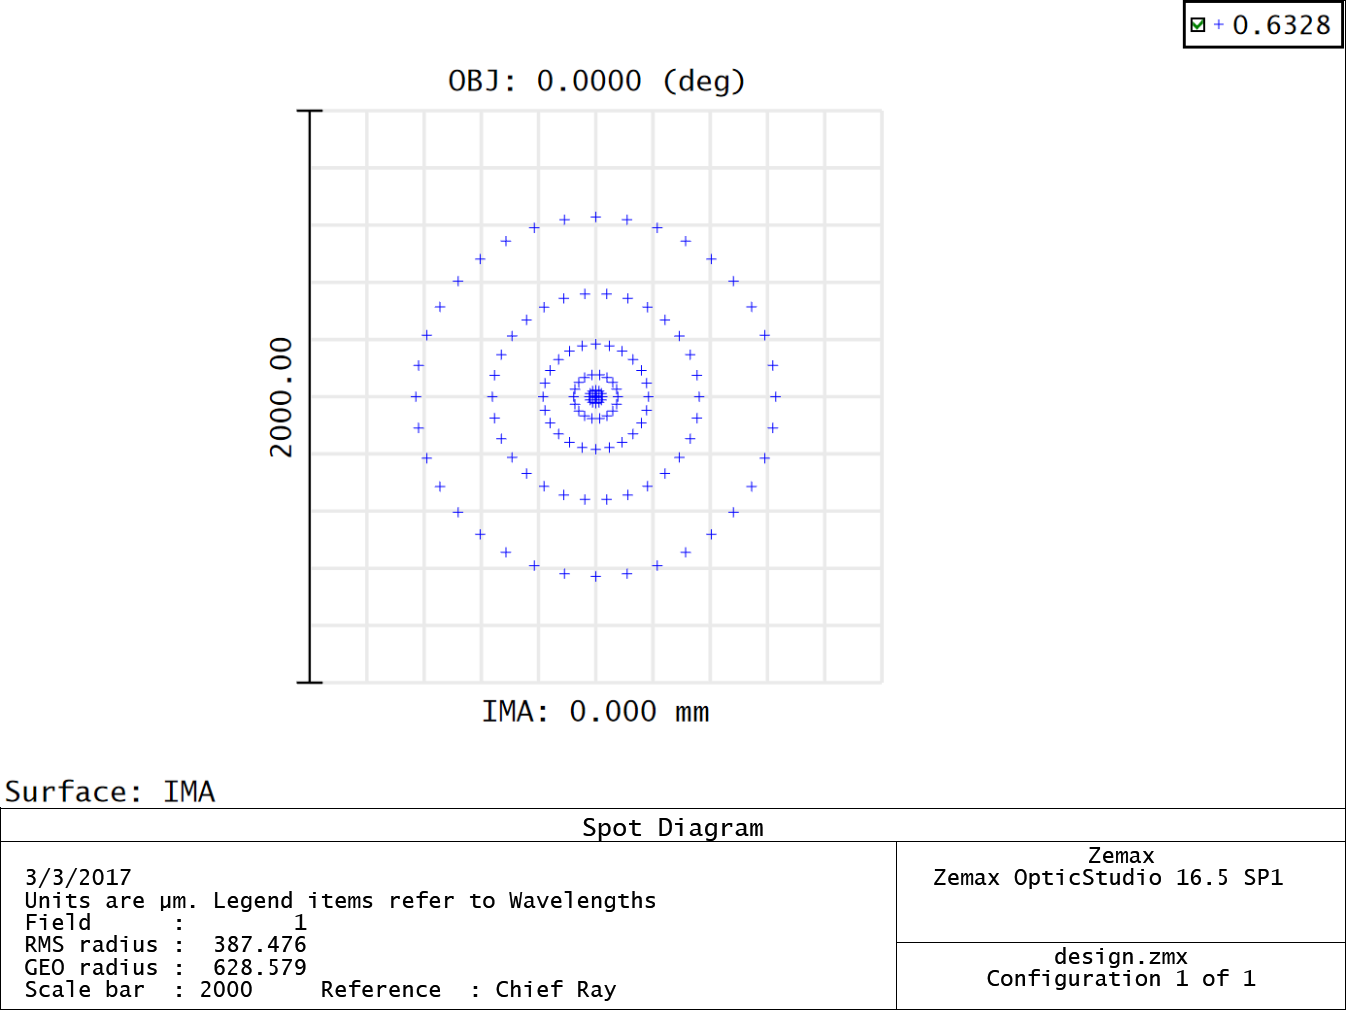
\includegraphics[trim={7.1cm 8.5cm 12cm 2.6cm}, clip,height=2.5cm]{../zemax/2_twoElement/2_optimize_RMS/spot.png} & \SI{792}{\milli \meter} &  \SI{387}{\micro \meter} \\\hline
		3 & split & 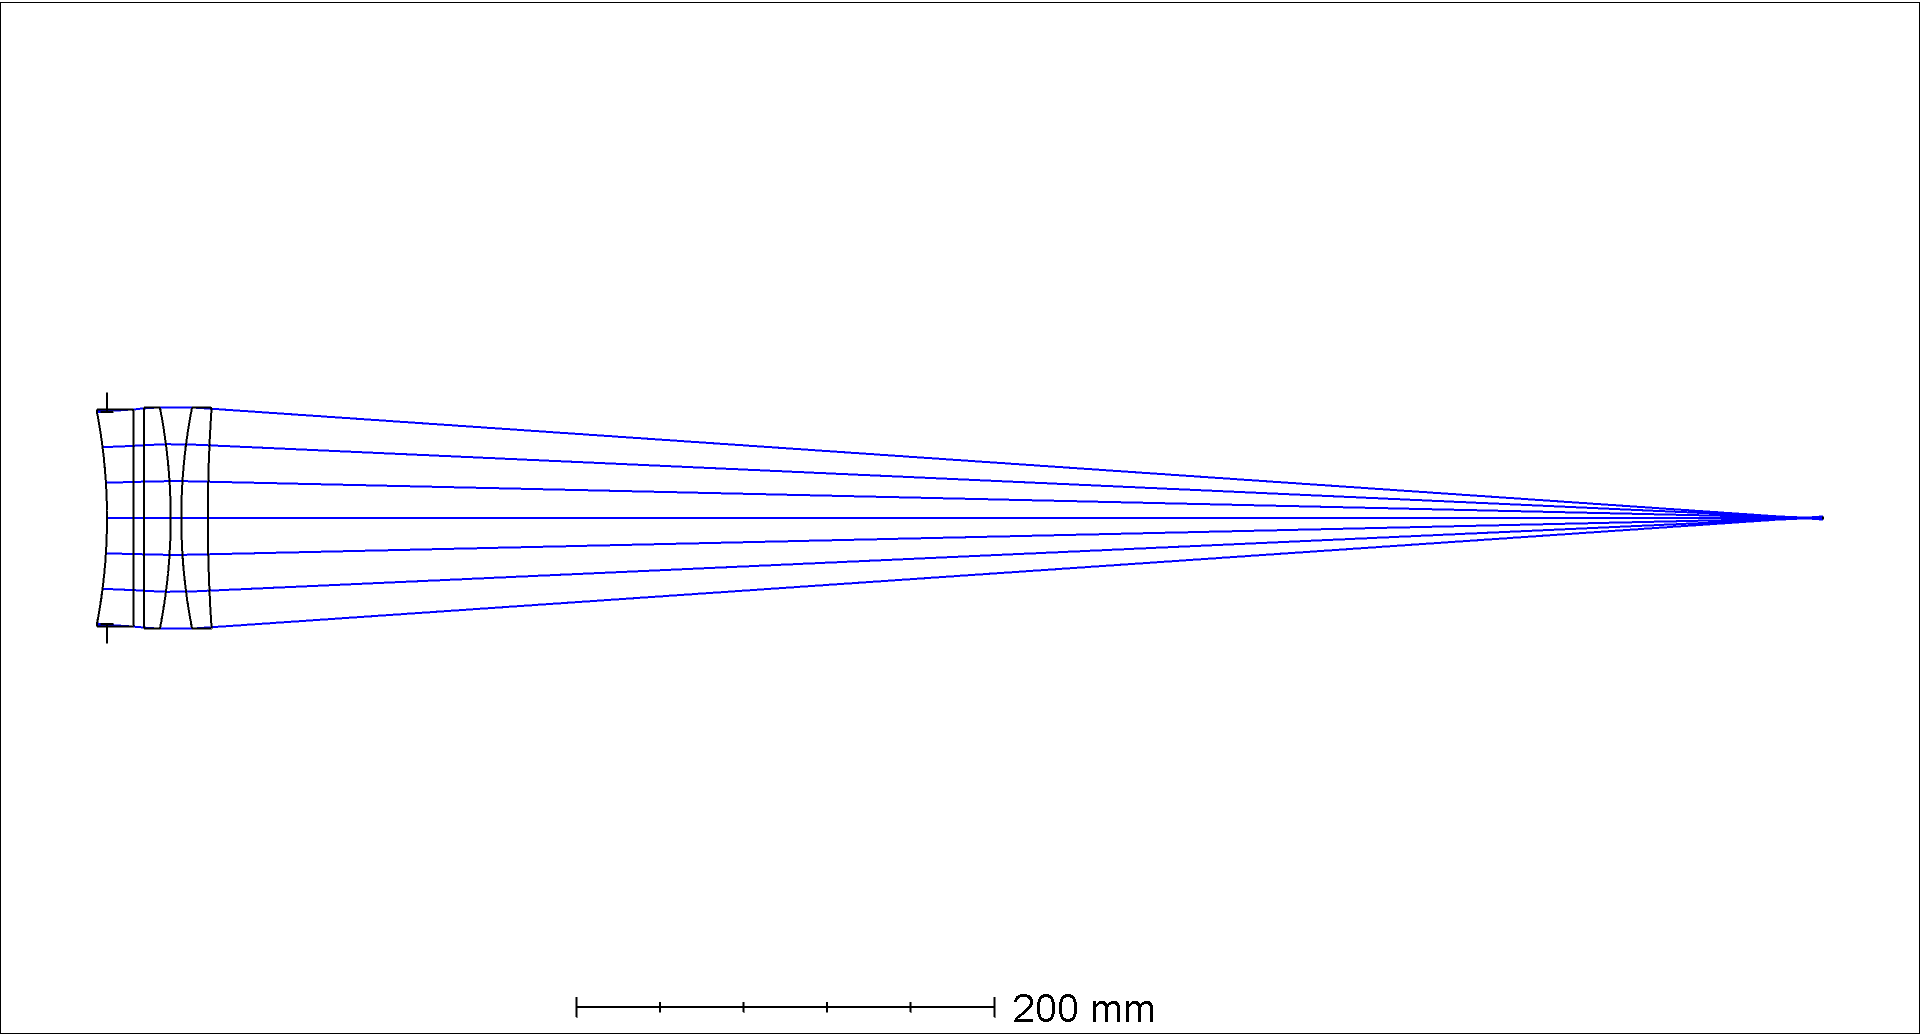
\includegraphics[trim={0.25cm 10cm 40cm 10cm}, clip,height=2.5cm]{../zemax/3_threeElement/1_initial/layout.png} & 
		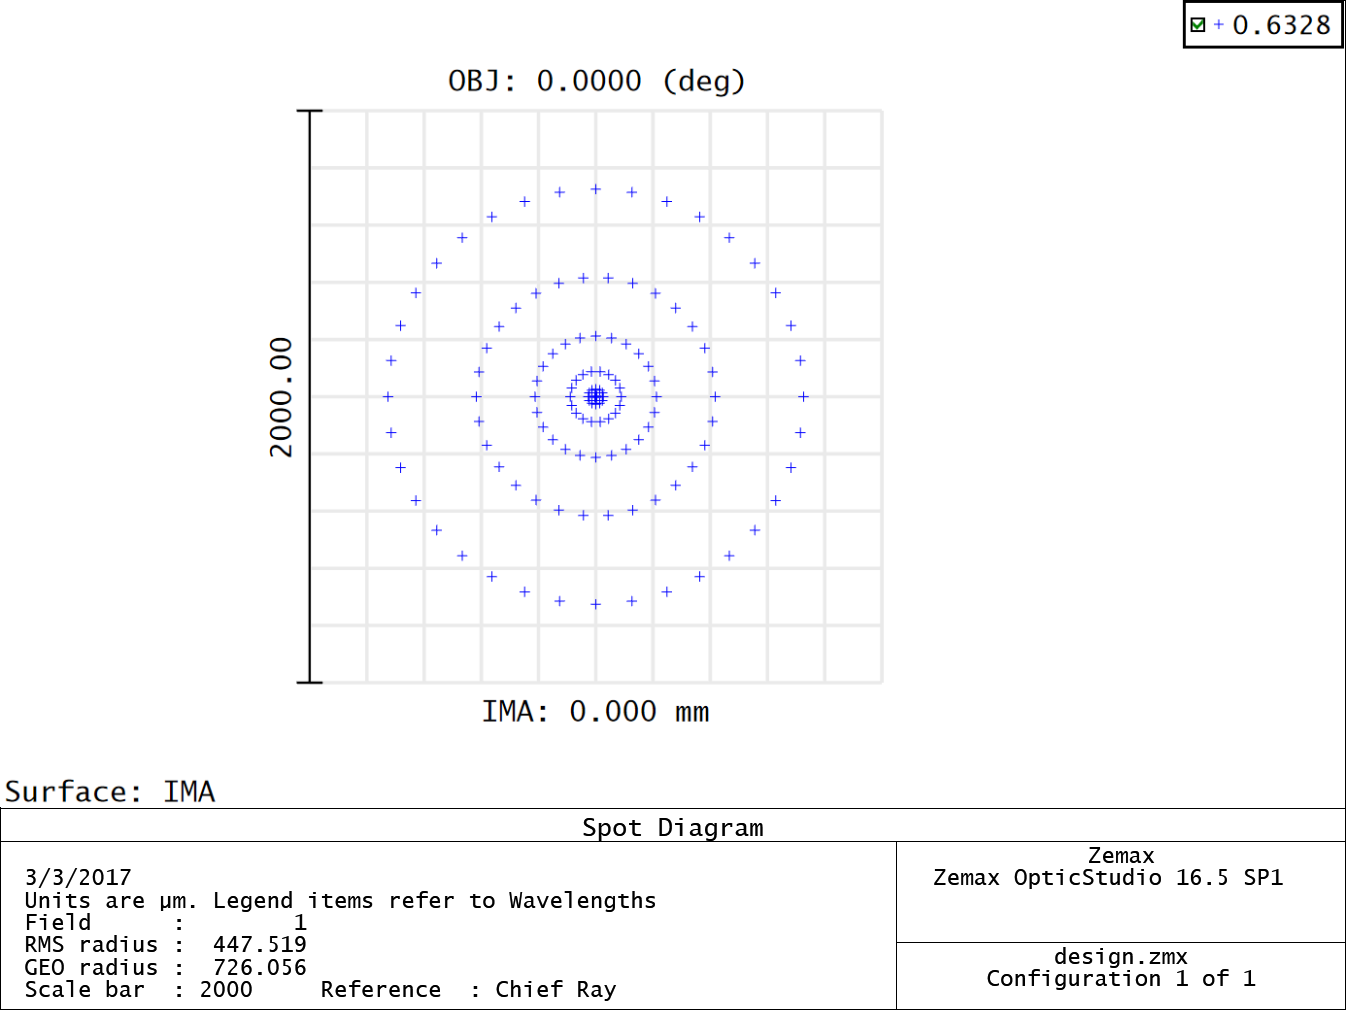
\includegraphics[trim={7.1cm 8.5cm 12cm 2.6cm}, clip,height=2.5cm]{../zemax/3_threeElement/1_initial/spot.png} & \SI{754}{\milli \meter} &  \SI{447}{\micro \meter} \\\hline
		3 & optimized & 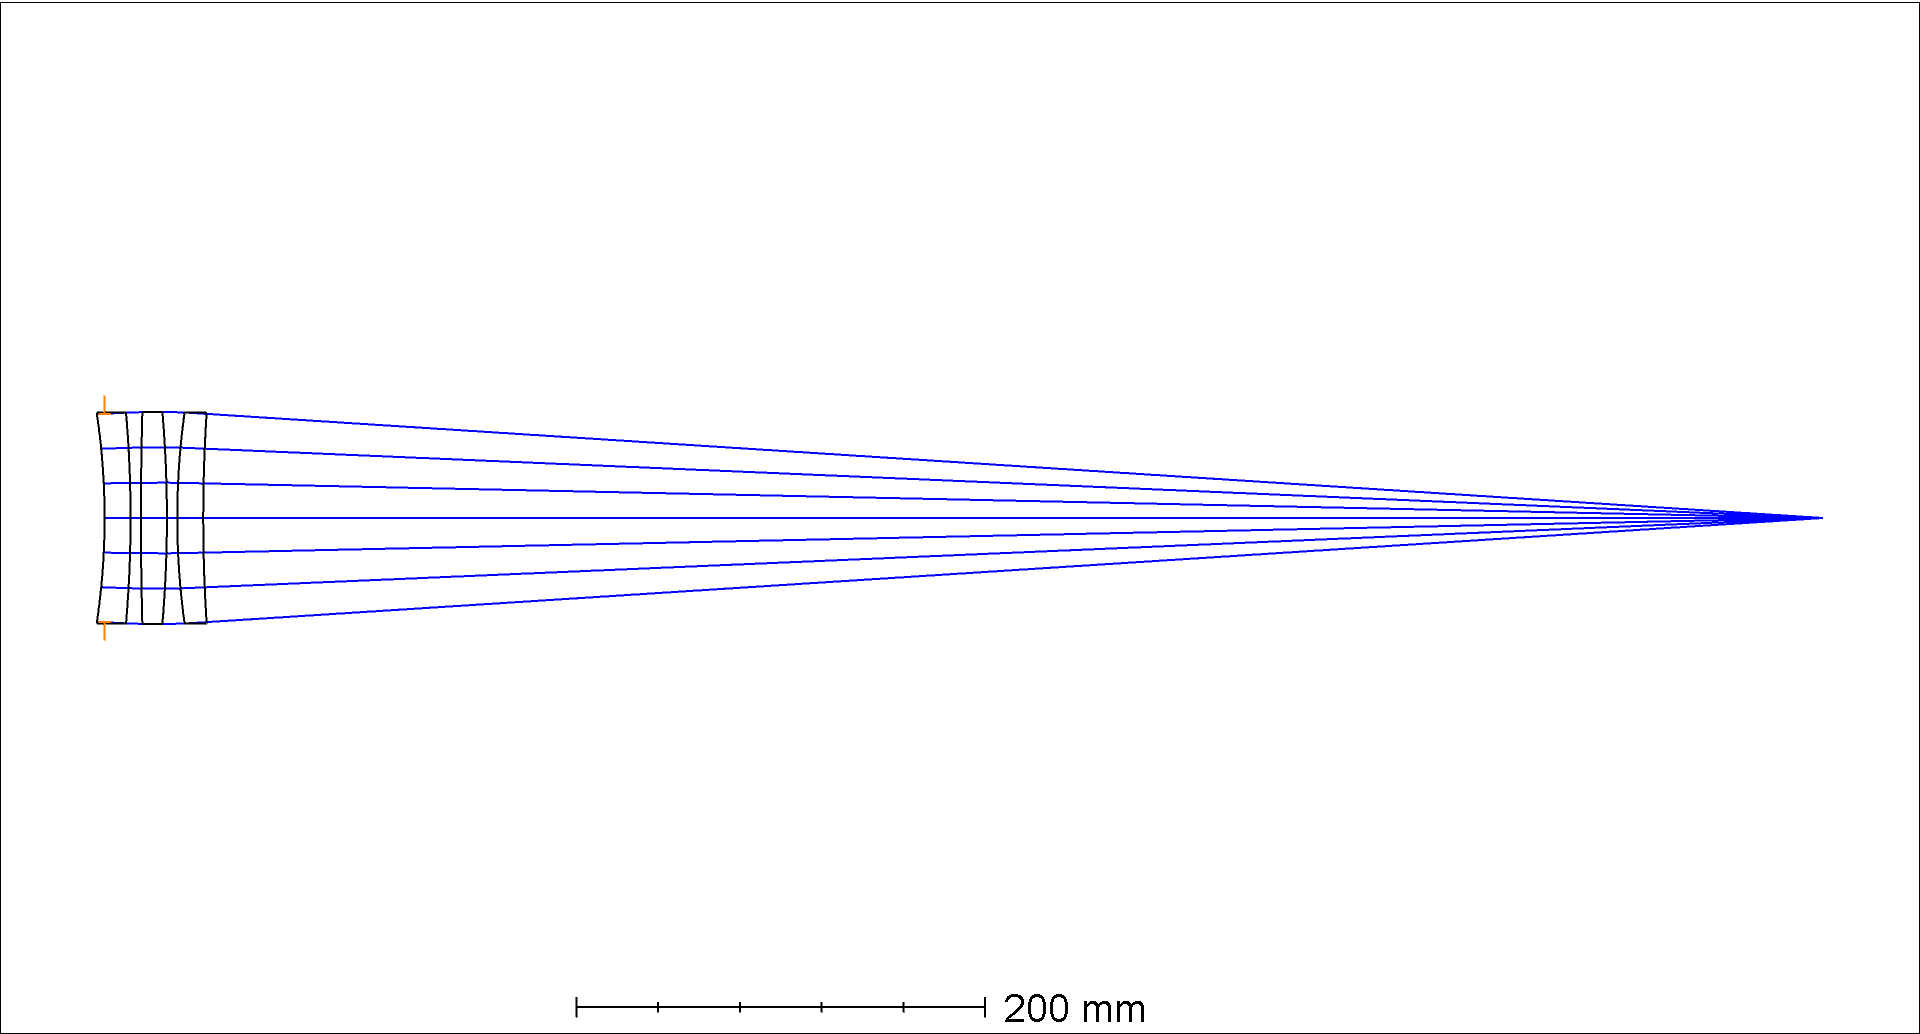
\includegraphics[trim={0.25cm 10cm 40cm 10cm}, clip,height=2.5cm]{../zemax/3_threeElement/2_optimize_RMS/layout.png} & 
		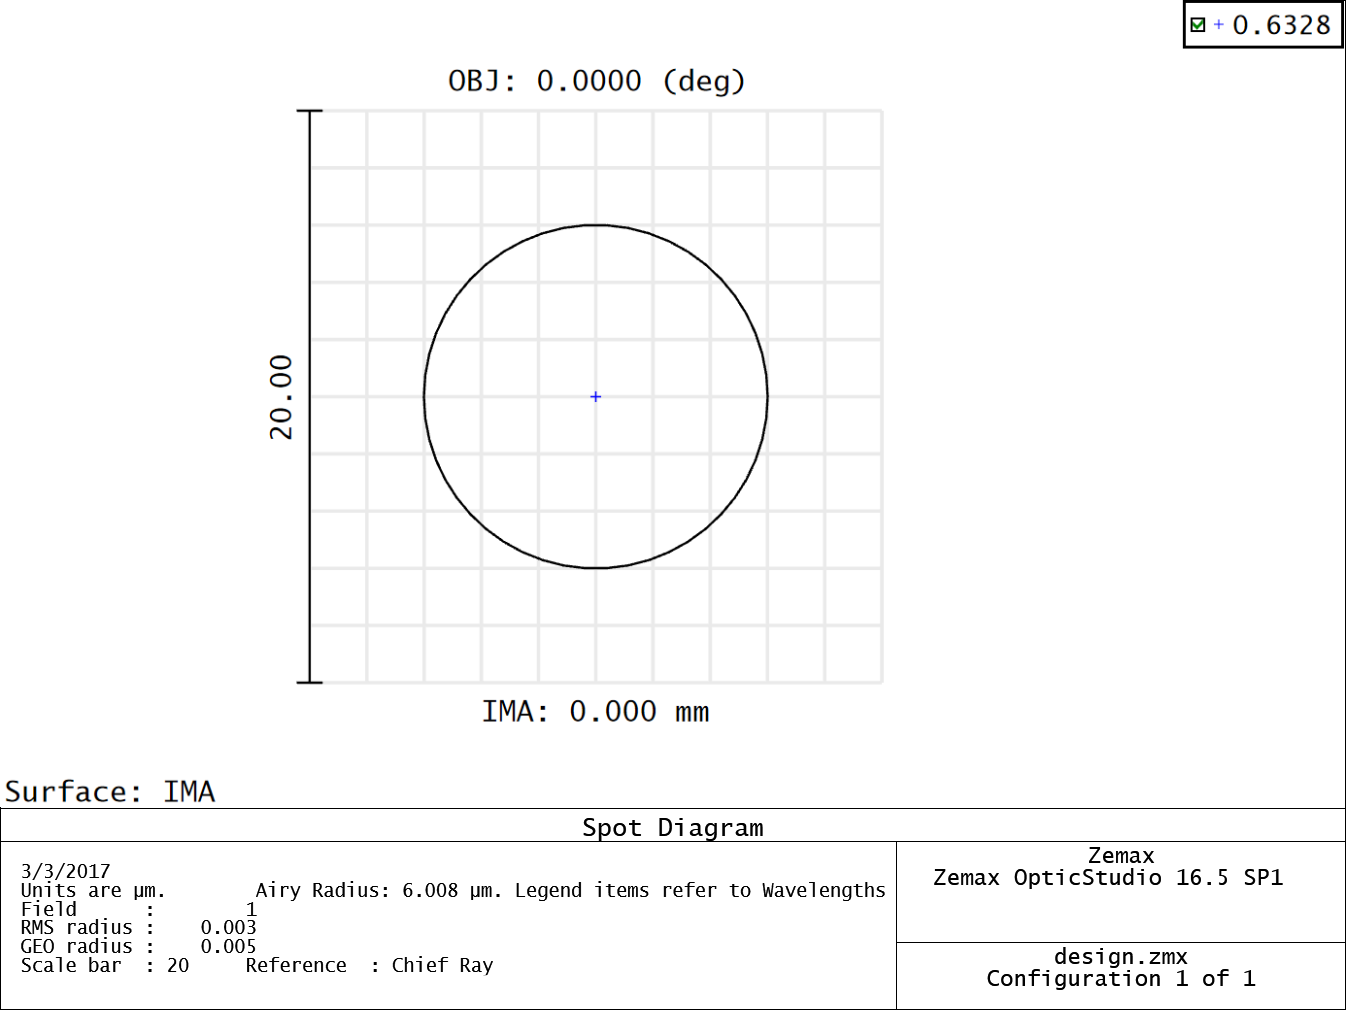
\includegraphics[trim={7.1cm 8.5cm 12cm 2.6cm}, clip,height=2.5cm]{../zemax/3_threeElement/2_optimize_RMS/spot.png} & \SI{792}{\milli \meter} &  \SI{0.003}{\micro \meter}	\\\hline		
	\end{tabular}
	\caption{Parameters for the optical design shown at each step.}	
	\label{opt}
\end{table}

\begin{figure}[h!]
	\centering
	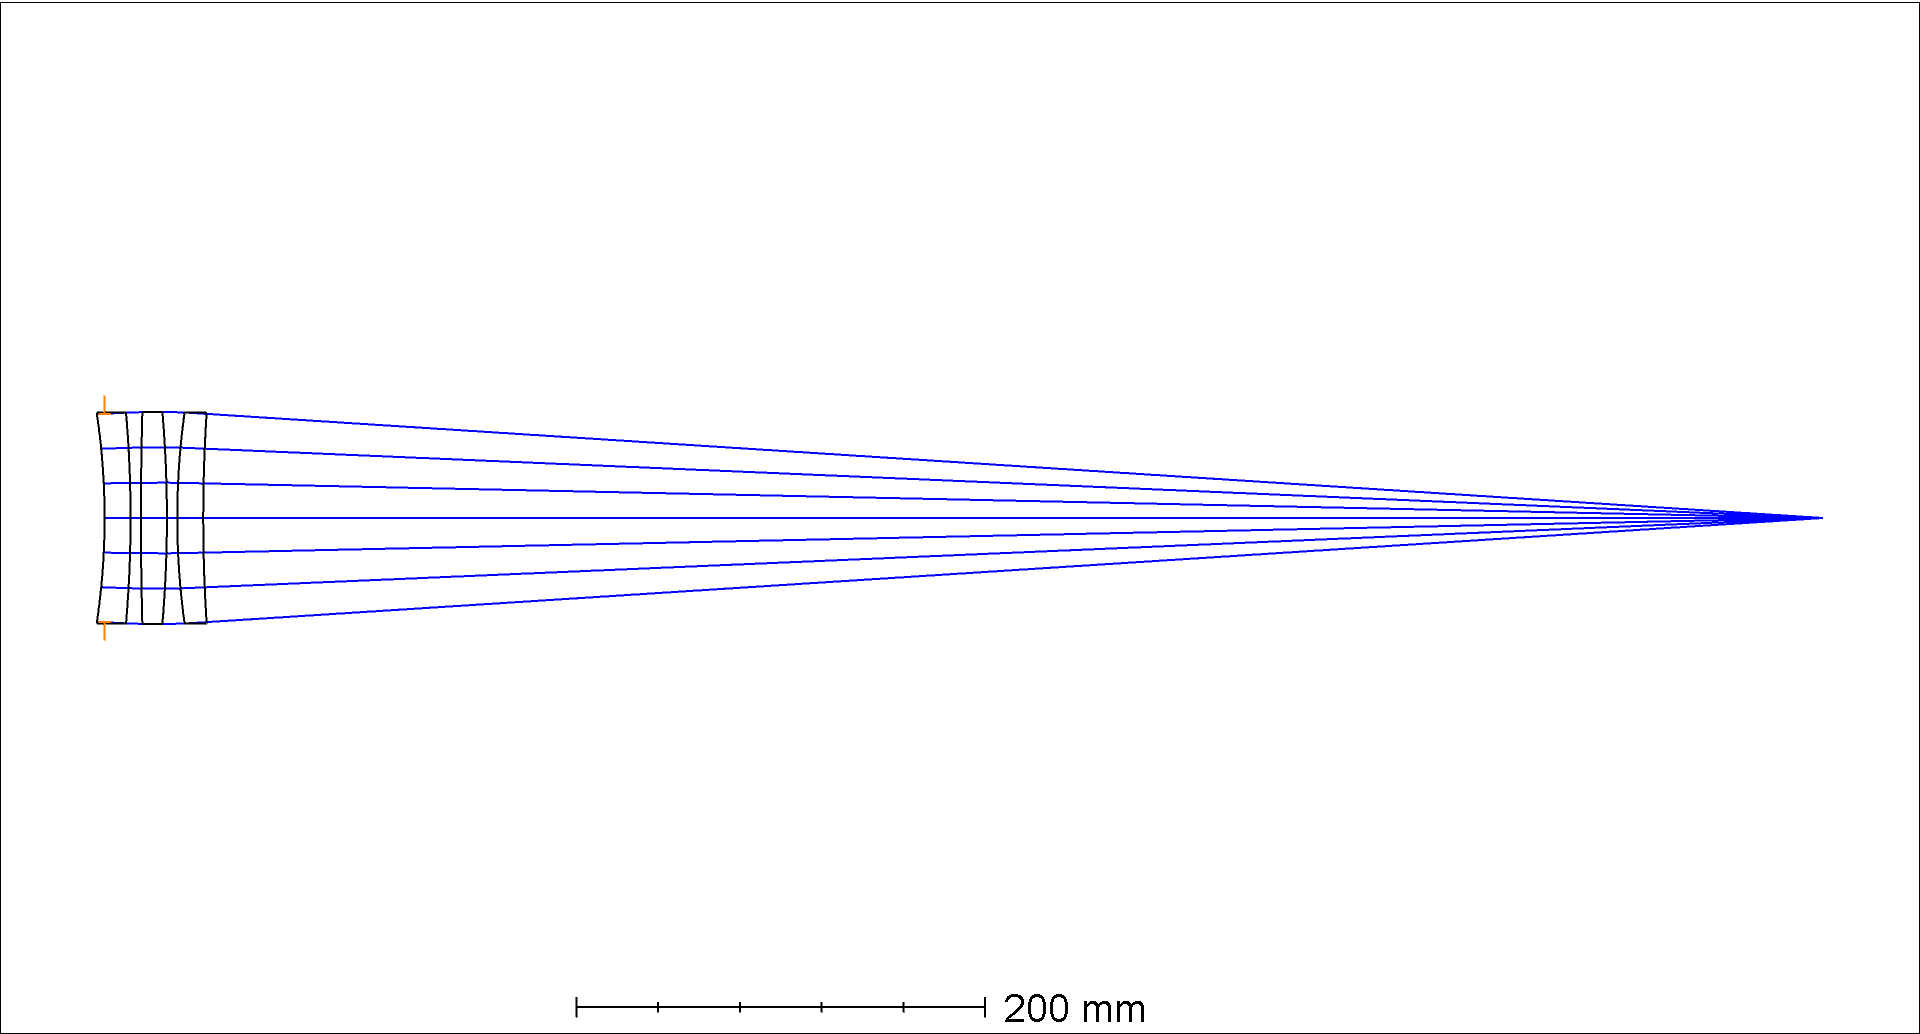
\includegraphics[width=0.75\linewidth]{../zemax/3_threeElement/2_optimize_RMS/layout}
	\caption{Layout of the final lens design}
\end{figure}

\begin{figure}[h!]
	\centering
	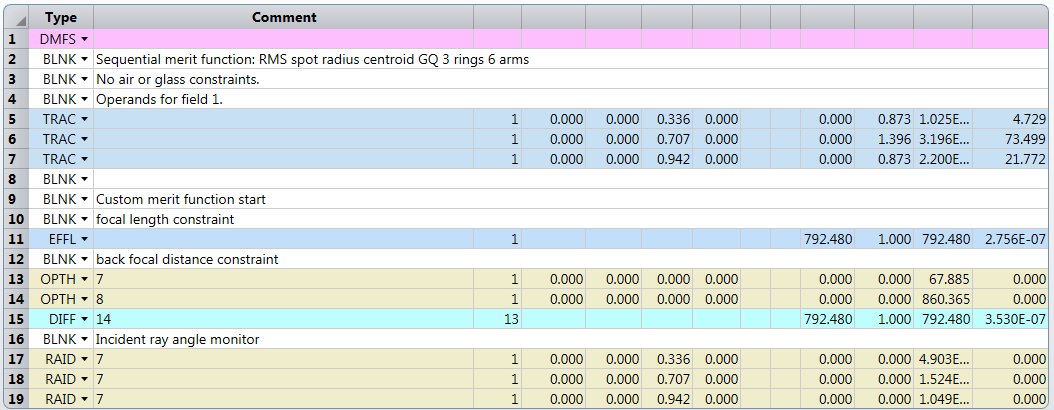
\includegraphics[width=0.75\linewidth]{../zemax/3_threeElement/2_optimize_RMS/merit}
	\caption{Merit function evaluated for the final lens design}
\end{figure}

\begin{figure}[h!]
	\centering
	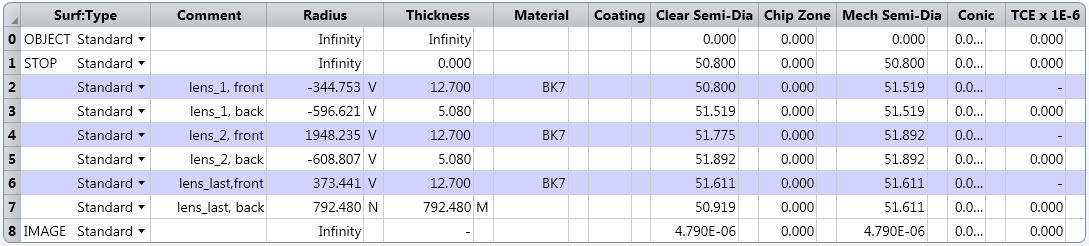
\includegraphics[width=0.75\linewidth]{../zemax/3_threeElement/2_optimize_RMS/lens}
	\caption{Lens prescription for the final lens design}
\end{figure}

\section{Final Design}

It took two lens splittings, resulting in a three lens optical system to achieve the desired EFFL, BFL, surface normal rays and diffraction limited performance described in the problem statement. Snapshots of the optimization process are given in Table \ref{opt}.

\end{document}
